\documentclass[border=2pt]{standalone}
\usepackage{mathptmx}
\usepackage{tikz}
\usetikzlibrary{positioning,arrows.meta,calc,fit,backgrounds,shapes.geometric}
\definecolor{ink}{HTML}{0B0B0B}
\definecolor{ink2}{HTML}{52514E}
\definecolor{muted}{HTML}{8A8A86}
\definecolor{panelbg}{HTML}{F6F5F1}
\definecolor{hair}{HTML}{DDDCD7}
\definecolor{cfind}{HTML}{1F8F5F}
\definecolor{ckeep}{HTML}{2F2F2C}
\definecolor{cclaim}{HTML}{D1A800}
\definecolor{cinf}{HTML}{E0561F}
\definecolor{cgain}{HTML}{9E1F3A}
\definecolor{backbone}{HTML}{EEEDE9}
\definecolor{lightblue}{HTML}{DFEBE2}
\tikzset{
  x=1pt, y=1pt, >={Stealth[length=3pt,width=2.6pt]},
  every node/.append style={font=\scriptsize, text=ink},
  box/.style={rounded corners=1.5pt, line width=0.55pt, minimum height=14pt, inner sep=1pt, align=center},
  trained/.style={box, draw=cinf, fill=cinf, text=white},
  frozen/.style={box, draw=cfind, fill=white},
  bb/.style={box, draw=muted, fill=backbone},
  off/.style={box, draw=muted, dashed, fill=white, text=muted},
  flow/.style={->, line width=0.6pt, draw=ink2},
  offflow/.style={->, line width=0.6pt, draw=muted, dash pattern=on 2pt off 1.6pt},
}
\begin{document}
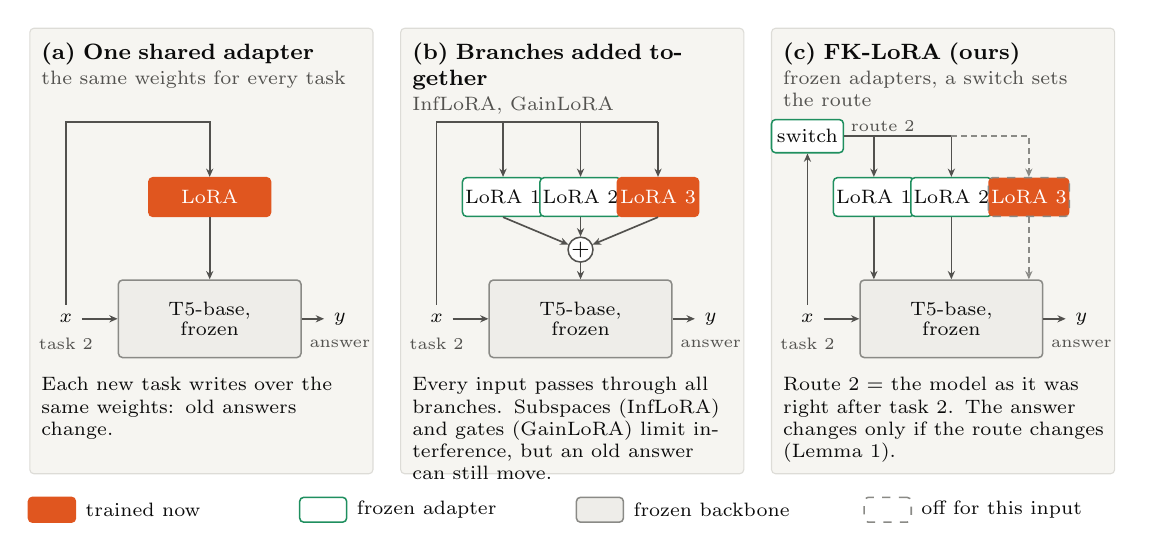
\begin{tikzpicture}[color=ink]
\def\W{124}\def\H{161}
% ---- panel frames
\foreach \i in {0,1,2}{
  \fill[panelbg, draw=hair, line width=0.4pt, rounded corners=1.5pt] (\i*134,0) rectangle (\i*134+\W,\H);
}
% ---- common sketch skeleton: x, block, y
\foreach \i in {0,1,2}{
  \begin{scope}[shift={(\i*134,0)}]
    \node[bb, minimum width=66pt, minimum height=28pt, text=ink] (blk\i) at (65,56) {T5-base,\\[-1pt]frozen};
    \node (x\i) at (13,56) {$x$};
    \node[text=ink2, font=\fontsize{6.5}{7}\selectfont] at (13,47) {task 2};
    \node (y\i) at (112,56) {$y$};
    \node[text=ink2, font=\fontsize{6.5}{7}\selectfont] at (112,47) {answer};
    \draw[flow] (x\i.east) -- (blk\i.west);
    \draw[flow] (blk\i.east) -- (y\i.west);
  \end{scope}
}
% ================= (a)
\begin{scope}[shift={(0,0)}]
  \node[anchor=north west, text width=116pt, inner sep=0] at (4,\H-5)
    {\footnotesize\bfseries (a) One shared adapter\\[1pt]\scriptsize\mdseries\color{ink2} the same weights for every task};
  \node[trained, minimum width=44pt] (a1) at (65,100) {LoRA};
  \draw[flow] (x0.north) -- ++(0,66) coordinate (r0) -- (r0 -| a1.north) -- (a1.north);
  \draw[flow] (a1.south) -- (blk0.north);
  \node[anchor=north west, text width=116pt, inner sep=0, align=left] at (4,35)
    {\scriptsize Each new task writes over the same weights: old answers change.};
\end{scope}
% ================= (b)
\begin{scope}[shift={(134,0)}]
  \node[anchor=north west, text width=116pt, inner sep=0] at (4,\H-5)
    {\footnotesize\bfseries (b) Branches added together\\[1pt]\scriptsize\mdseries\color{ink2} InfLoRA, GainLoRA};
  \node[frozen, minimum width=26pt] (b1) at (37,100) {LoRA 1};
  \node[frozen, minimum width=26pt] (b2) at (65,100) {LoRA 2};
  \node[trained, minimum width=26pt] (b3) at (93,100) {LoRA 3};
  \node[circle, draw=ink2, line width=0.55pt, inner sep=0pt, minimum size=9pt, fill=white] (pl) at (65,81) {\footnotesize $+$};
  \draw[line width=0.6pt, draw=ink2] (x1.north) -- ++(0,66) coordinate (r1) -- (r1 -| b3.north);
  \foreach \b in {b1,b2,b3}{ \draw[flow] (r1 -| \b.north) -- (\b.north); \draw[flow] (\b.south) -- (pl); }
  \draw[flow] (pl) -- (blk1.north);
  \node[anchor=north west, text width=116pt, inner sep=0, align=left] at (4,35)
    {\scriptsize Every input passes through all branches. Subspaces (\mbox{InfLoRA}) and gates (\mbox{GainLoRA}) limit interference, but an old answer can still move.};
\end{scope}
% ================= (c)
\begin{scope}[shift={(268,0)}]
  \node[anchor=north west, text width=116pt, inner sep=0] at (4,\H-5)
    {\footnotesize\bfseries (c) FK-LoRA (ours)\\[1pt]\scriptsize\mdseries\color{ink2} frozen adapters, a switch sets the route};
  \node[frozen, minimum width=26pt] (c1) at (37,100) {LoRA 1};
  \node[frozen, minimum width=26pt] (c2) at (65,100) {LoRA 2};
  \node[trained, draw=muted, dashed, minimum width=26pt] (c3) at (93,100) {LoRA 3};
  \node[frozen, minimum width=26pt, minimum height=12pt] (sw) at (13,122) {switch};
  \draw[flow] (x2.north) -- (sw.south);
  \draw[flow] (sw.east) -- ++(11,0) coordinate (r2) -- (r2 -| c1.north) -- (c1.north);
  \draw[flow] (r2 -| c1.north) -- (r2 -| c2.north) -- (c2.north);
  \draw[offflow] (r2 -| c2.north) -- (r2 -| c3.north) -- (c3.north);
  \node[font=\fontsize{6.5}{7}\selectfont, text=ink2, anchor=south west, inner sep=0.5pt] at (28,123) {route 2};
  \draw[flow] (c1.south) -- (c1.south |- blk2.north);
  \draw[flow] (c2.south) -- (c2.south |- blk2.north);
  \draw[offflow] (c3.south) -- (c3.south |- blk2.north);
  \node[anchor=north west, text width=116pt, inner sep=0, align=left] at (4,35)
    {\scriptsize Route 2 = the model as it was right after task 2. The answer changes only if the route changes (Lemma~1).};
\end{scope}
% ---- legend
\begin{scope}[shift={(0,-13)}]
  \node[trained, minimum width=17pt, minimum height=9pt] at (8,0) {};
  \node[anchor=west, inner sep=0] at (20,0) {trained now};
  \node[frozen, minimum width=17pt, minimum height=9pt] at (106,0) {};
  \node[anchor=west, inner sep=0] at (118,0) {frozen adapter};
  \node[bb, minimum width=17pt, minimum height=9pt] at (206,0) {};
  \node[anchor=west, inner sep=0] at (218,0) {frozen backbone};
  \node[off, minimum width=17pt, minimum height=9pt] at (310,0) {};
  \node[anchor=west, inner sep=0] at (322,0) {off for this input};
\end{scope}
\end{tikzpicture}
\end{document}
